\section{Test Processor Completely (Test Complet du Processeur)}
\label{sec:Test Processor Completely (Test Complet du Processeur)}
In this part, we will test the processor complement.

We first change the code Assembly given to the instruction code in \textbf{instruction\_memory2.vhd} according to Figure \ref{fig:AISF}.
\begin{lstlisting}[style = vhdl,columns=fixed]
result (0):=x"E3A00010";  -- 0x0 _main   -- MOV R0,#0x10
result (1):=x"E3A01001";  -- 0x1		 -- MOV R1,#0x01
result (2):=x"E6103000";  -- 0x2 _for    -- LDR R3,[R0]
result (3):=x"E6104001";  -- 0x3		 -- LDR R4,[R0,#1]
result (4):=x"E6004000";  -- 0x4		 -- STR R4,[R0]
result (5):=x"E6003001";  -- 0x5		 -- STR R3,[R0,#1]
result (6):=x"E2811001";  -- 0x6		 -- ADD R1,R1,#1
result (7):=x"E2800001";  -- 0x7		 -- ADD R0,R0,#1
result (8):=x"E351000A";  -- 0x8		 -- CMP R1,0xA
result (9):=x"BAFFFFF8";  -- 0x9		 -- BLT loop
result (10):=x"EAFFFFFF"; -- 0xA _wait	 -- BAL wait
\end{lstlisting}

After runing the simulation with command file \textbf{Processor\_test.do}, we obtaine waves as Figure \ref{fig:PUCres}.
Detailed waves can be found as Figure \ref{fig:ModelSim_ processeur_tb(bench) C} in Appendices \ref{AppendicesA}.

\begin{figure}[htp]
    \centering
    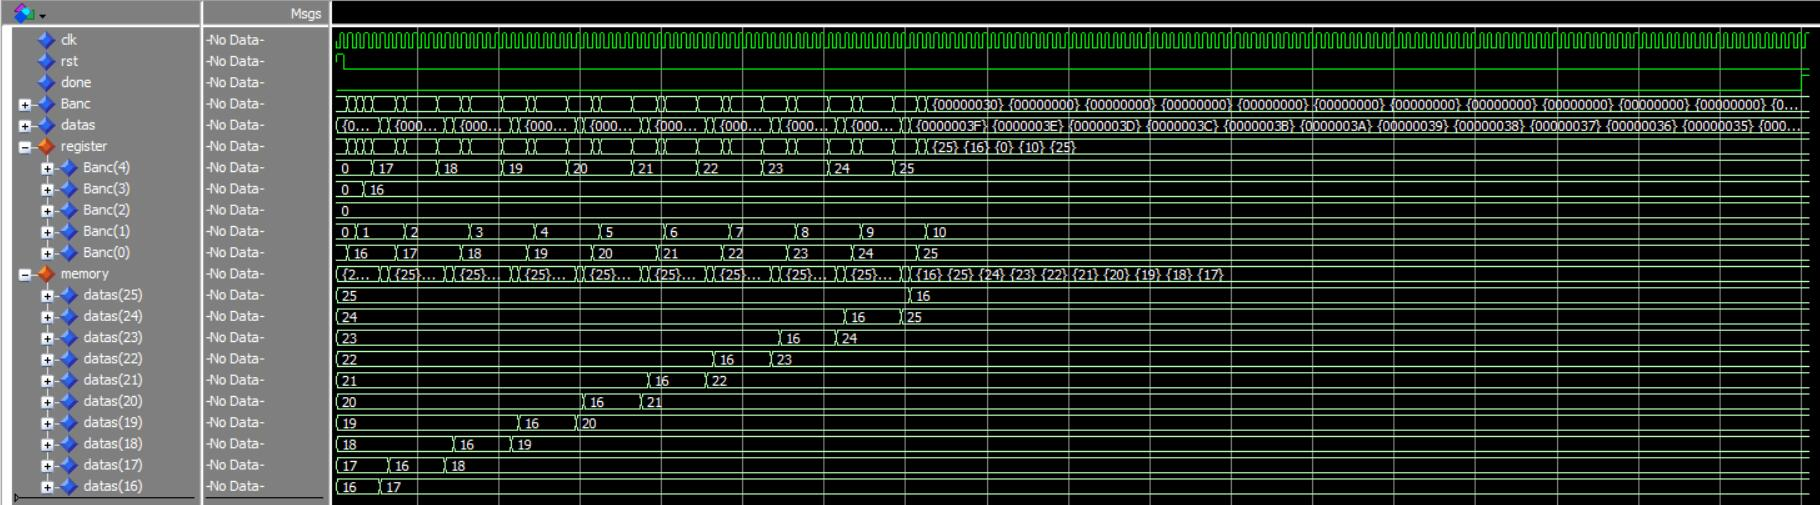
\includegraphics[width=1\textwidth]{picture/PUCres.jpg}
    \caption{Simulation Waves of Processing Unit Completely}     
    \label{fig:PUCres}
\end{figure}